% TEMPLATE.TEX
%
% Time-stamp: <2013-03-26 11:09 olenz>
%
% This is an extensively documented LaTeX file that shows how to
% produce a good-looking document with current LaTeX (11/2012).
%
% IMPORTANT!
%
%   Some obsolete commands and packages
% ----------|-------------------------------
% obsolete  |     Replacement in LATEX 2ε
% ----------|-------------------------------
%           | local            global/switch
% ----------|-------------------------------
% {\bf ...} | \textbf{...}     \bfseries
%     -     | \emph{...}       \em
% {\it ...} | \textit{...}     \itshape
%     -     | \textmd{...}     \mdseries
% {\rm ...} | \textrm{...}     \rmfamily
% {\sc ...} | \textsc{...}     \scshape
% {\sf ...} | \textsf{...}     \sffamily
% {\sl ...} | \textsl{...}     \slshape
% {\tt ...} | \texttt{...}     \ttfamily
%     -     | \textup{...}     \upshape
%
% DON'T USE \\ TO MAKE LINEBREAKS, INSTEAD JUST LEAVE A BLANK LINE!
%
\RequirePackage[l2tabu,orthodox]{nag} % turn on warnings because of bad style
\documentclass[a4paper,10pt,bibtotoc]{scrartcl}
%
\usepackage[bottom=3.5cm, top=3cm]{geometry}
%%%%%%%%%%%%%%%%%%%%%%%%%%%%%%%%%%%%
% KOMA CLASSES
%%%%%%%%%%%%%%%%%%%%%%%%%%%%%%%%%%%%
%
% The class "scrartcl" is one of the so-called KOMA-classes, a set of
% very well done LaTeX-classes that produce a very European layout
% (e.g. titles with a sans-serif font).
%
% The KOMA classes have extensive documentation that you can access
% via the commands:
%   texdoc scrguide # in German
%   texdoc scrguien # in English
%
%
% The available classes are:
%
% scrartcl - for "articles", typically for up to ~20 pages, the
%            highest level sectioning command is \section
%
% scrreprt - for "reports", typically for up to ~200 pages, the
%            highest level sectioning command is \chapter
%
% scrbook  - for "books", for more than 200 pages, the highest level
%            sectioning command is \part.
%
% USEFUL OPTIONS
%
% a4paper  - Use a4 paper instead of the default american letter
%            format.
%
% 11pt, 12pt, 10pt
%          - Use a font with the given size.
%
% bibtotoc - Add the bibliography to the table of contents
%
% The KOMA-script classes have plenty of options to modify

% This allows to type UTF-8 characters like ä,ö,ü,ß
\usepackage[utf8]{inputenc}

\usepackage[T1]{fontenc}        % Tries to use Postscript Type 1 Fonts for better rendering
\usepackage{lmodern}            % Provides the Latin Modern Font which offers more glyphs than the default Computer Modern
\usepackage[intlimits]{amsmath} % Provides all mathematical commands

\usepackage{hyperref}           % Provides clickable links in the PDF-document for \ref
\usepackage{graphicx}            % Allow you to include images (like graphicx). Usage: \includegraphics{path/to/file}

% Allows to set units
\usepackage[ugly]{units}        % Allows you to type units with correct spacing and font style. Usage: $\unit[100]{m}$ or $\unitfrac[100]{m}{s}$

% Additional packages
\usepackage{url}                % Lets you typeset urls. Usage: \url{http://...}
\usepackage{breakurl}           % Enables linebreaks for urls
\usepackage{xspace}             % Use \xpsace in macros to automatically insert space based on context. Usage: \newcommand{\es}{ESPResSo\xspace}
\usepackage{xcolor}             % Obviously colors. Usage: \color{red} Red text
\usepackage{booktabs}           % Nice rules for tables. Usage \begin{tabular}\toprule ... \midrule ... \bottomrule
\usepackage{siunitx}


% Source code listings
\usepackage{listings}           % Source Code Listings. Usage: \begin{lstlisting}...\end{lstlisting}
\lstloadlanguages{python}
\definecolor{lightpurple}{rgb}{0.8,0.8,1}

\lstset{
stepnumber=1,
numbersep=5pt,
numberstyle=\small\color{black},
basicstyle=\ttfamily,
%keywordstyle=\color{black},
%commentstyle=\color{black},
%stringstyle=\color{black},
frame=single,
tabsize=4,
language = python,
backgroundcolor=\color{black!5}}

\usepackage{float}

\begin{document}

\titlehead{Simulation Methods in Physics I \hfill WS 2019/2010}
\title{Report for Worksheet 2: Statistical Mechanics and Molecular Dynamics}
\author{Markus Baur and David Beyer}
\date{\today}
%\publishers{Institute for Computational Physics, University of Stuttgart}
\maketitle

\tableofcontents

\section{Statistical Mechanics}
\subsection{Entropy}
To calculate the entropy of the combined system, we make use of the statistical mechanical assumption that the number of available states is multiplicative for large enough systems. 
This leads to a total number of
\begin{align}
 \Omega = \Omega_1\cdot\Omega_2 = 10^{31}\cdot 10^{28}= 10^{59}
\end{align}
configurations. 
The entropies are given by
\begin{align*}
S_1 &= k_\mathrm{B}\cdot \mathrm{ln}\left(\Omega_1\right) \approx \SI[per-mode=reciprocal]{6.15e-3}{\electronvolt\per\kelvin}\\
S_2 &= k_\mathrm{B}\cdot \mathrm{ln}\left(\Omega_2\right) \approx \SI[per-mode=reciprocal]{5.56e-3}{\electronvolt\per\kelvin}\\
S &= k_\mathrm{B}\cdot \mathrm{ln}\left(\Omega\right) = k_\mathrm{B}\cdot \mathrm{ln}\left(\Omega_1\right) + k_\mathrm{B}\cdot \mathrm{ln}\left(\Omega_2\right) = S_1 + S_2\approx \SI[per-mode=reciprocal]{11.2e-3}{\electronvolt\per\kelvin}.
\end{align*}
The increase in the number of configurations can be calculated using the increase of the entropy.
To calculate entropy differences, we make use of the fundamental thermodynamic relation
\begin{align}
\mathrm{d}S = \frac{1}{T}\mathrm{d}U + \frac{p}{T}\mathrm{d}V - \frac{\mu}{T}\mathrm{d}N.
\end{align}
Treating neon as a monatomic, ideal gas we have
\begin{align}
 pV &= Nk_\mathrm{B}T\\
 U &= \frac{3N}{2}k_\mathrm{B} T.
\end{align}
For the expansion at constant temperature and particle number we have
\begin{align}
 \mathrm{d}S = \frac{1}{T}\underbrace{\mathrm{d}U}_{=0} + \frac{p}{T}\mathrm{d}V - \frac{\mu}{T}\underbrace{\mathrm{d}N}_{=0} = \frac{Nk_\mathrm{B}}{V}\mathrm{d}V = \frac{p_\mathrm{i} V_\mathrm{i}}{T}\cdot\frac{\mathrm{d}V}{V}
\end{align}
which can be integrated to give the entropy difference $\Delta S$:
\begin{align}
 \Delta S = \int_{S_\mathrm{i}}^{S_\mathrm{f}}\,\mathrm{d}S = \frac{p_\mathrm{i} V_\mathrm{i}}{T}\int_{V_\mathrm{i}}^{V_\mathrm{f}}\,\frac{\mathrm{d} V}{V} = \frac{p_\mathrm{i} V_\mathrm{i}}{T}\ln\left(\frac{V_\mathrm{f}}{V_\mathrm{i}}\right) = \frac{p_\mathrm{i} V_\mathrm{i}}{T}\ln\left(1.01\right)
\end{align}
The entropy difference can also be expressed as a function of the inital and final number of configurations:
\begin{align}
\Delta S = k_\mathrm{B}\ln\left(\frac{\Omega_\mathrm{f}}{\Omega_\mathrm{i}}\right).
\end{align}
Using this relationship, we can express the $\Omega_\mathrm{f}$ in the following way:
\begin{align}
 \Omega_\mathrm{f} = \Omega_\mathrm{i}\cdot e^{\frac{\Delta S}{k_\mathrm{B}}} \approx 1.01\cdot \exp\left(2.463\cdot 10^{25}\right)\cdot \Omega_\mathrm{i}.
\end{align}
For the addition of energy at constant volume and particle number we have
\begin{align}
 \mathrm{d}S = \frac{1}{T}\mathrm{d}U + \frac{p}{T}\underbrace{\mathrm{d}V}_{=0} - \frac{\mu}{T}\underbrace{\mathrm{d}N}_{=0} = \frac{3Nk_\mathrm{B}}{2}\cdot\frac{\mathrm{d}U}{U}.
\end{align}
Integrating this relation results in
\begin{align}
 \Delta S = \int_{S_\mathrm{i}}^{S_\mathrm{f}}\,\mathrm{d}S = \frac{3Nk_\mathrm{B}}{2}\int_{U_\mathrm{i}}^{U_\mathrm{f}}\,\frac{\mathrm{d} U}{U} = \frac{3Nk_\mathrm{B}}{2}\ln\left(\frac{U_\mathrm{f}}{U_\mathrm{i}}\right) = \frac{3Nk_\mathrm{B}}{2}\ln\left(\frac{\frac{3Nk_\mathrm{B}}{2}T_\mathrm{i} + 100\,\mathrm{kJ}}{\frac{3Nk_\mathrm{B}}{2}T_\mathrm{i}}\right)
\end{align}
which gives us
\begin{align}
 \Omega_\mathrm{f} = \Omega_\mathrm{i}\cdot e^{\frac{\Delta S}{k_\mathrm{B}}} \approx 21\cdot \exp\left(9.03\cdot 10^{23}\right)\cdot \Omega_\mathrm{i}.
\end{align}


\subsection{Thermodynamic Variables in the Canonical Ensemble}
From the perspective of equilibrium statistical mechanics, all information about the system is contained in the partition function 
\begin{align}
 Z = \int\frac{\mathrm{d}\Gamma}{h^{3N}N!}\cdot e^{-\beta H}.
\end{align}
The internal energy $U$ is the expectation value of the Hamiltonian $H$, given by
\begin{align}
 U = \langle H\rangle = \int\frac{\mathrm{d}\Gamma}{Zh^{3N}N!}\cdot H\cdot e^{-\beta H}.
\end{align}
This can also be written as a derivative:
\begin{align}
 U = -\frac{\partial_\beta Z}{Z} =-\partial_\beta\ln\left(Z\right) = \partial_\beta\left(\beta F\right).
\end{align}
To calculate the pressure, we make use of the fundamental thermodynamic relation
\begin{align}
 \mathrm{d}F = -S\mathrm{d}T - p\mathrm{d}V + \mu\mathrm{d}N,
\end{align}
giving us
\begin{align}
p = -\partial_V F = \partial_V\left(\frac{Z}{\beta}\right).
\end{align}
Similarly, the entropy can be calculated as
\begin{align}
 S = -\partial_T F = k_\mathrm{B}\ln\left( Z\right) + k_\mathrm{B}T \frac{\partial_T Z}{Z} = k_\mathrm{B}\left(\ln\left( Z\right)  -\beta \partial_\beta \ln\left(Z\right)\right)
\end{align}.



\subsection{Ideal Gas}
The free energy of the ideal gas is given by
\begin{align}
\begin{split}
 F &= -\frac{1}{\beta}\ln\left(Z\right) = -\frac{1}{\beta}\ln\left(\frac{V^N}{\lambda^{3N}N!} \right) \approx  -\frac{1}{\beta}\left(\ln\left(\frac{V^N}{\lambda^{3N}}\right) -N\ln\left(N\right) + N\right)\\
 &= -\frac{N}{\beta}\left(\ln\left(\frac{V}{\lambda^{3}N}\right) + 1\right).
\end{split}
\end{align}
The use of the Stirling approximation is valid in the thermodynamic limit $N\rightarrow \infty$.
The heat capacity at constant volume is defined as
\begin{align}
C_V = \left( \frac{\partial U}{\partial T}\right)_V{V,N}.
\end{align}
We can calculate the internal energy using the result of the previous problem:
\begin{align}
 U = -\partial_\beta \ln\left(Z\right) =\frac{3N}{2}\cdot\frac{\partial_\beta \beta}{\beta} = \frac{3N}{2} k_\mathrm{B}T.
\end{align}
This leads to
\begin{align}
C_V = \frac{3N}{2} k_\mathrm{B}.
\end{align}
The pressure is given by
\begin{align}
p = -\partial_V F = \frac{N}{\beta}\partial_V\left(\ln\left(\frac{V}{\lambda^{3}N}\right) + 1\right) = \frac{N}{\beta V} = \frac{Nk_\mathrm{B}T}{V}.
\end{align}

\section{Molecular Dynamics: Lennard-Jones Fluid}
\subsection{Lennard-Jones Potential}
The function to calculate the Lennard-Jones potential was implemented in the following way:
\begin{lstlisting}
def lj_potential(r_ij):
    ret = 4 * (1/np.linalg.norm(r_ij)**12 \
        - 1/np.linalg.norm(r_ij)**6)
    return ret
\end{lstlisting}
A plot is shown in \autoref{fig:fig1}.

The function to calculate the $x$-component of the Lennard-Jones force was implemented in the following way:
\begin{lstlisting}
def lj_force(r_ij):
    ret = 24.0 * (2.0/np.linalg.norm(r_ij)**14 \
        - 1/np.linalg.norm(r_ij)**8) * r_ij
    return ret
\end{lstlisting}
A plot is shown in \autoref{fig:fig2}.

\begin{figure}[t]
 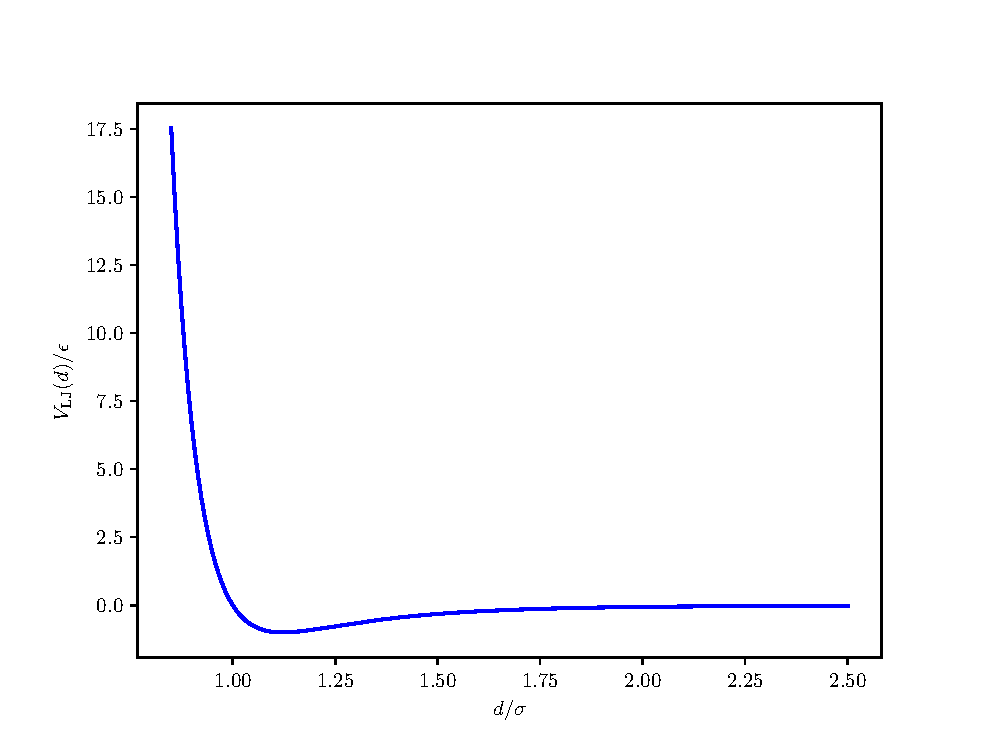
\includegraphics{lennard_jones_potential.eps}
 \caption{Plot of the Lennard-Jones potential as a function of the distance $d$.}
 \label{fig:fig1}
\end{figure}
\begin{figure}[t]
 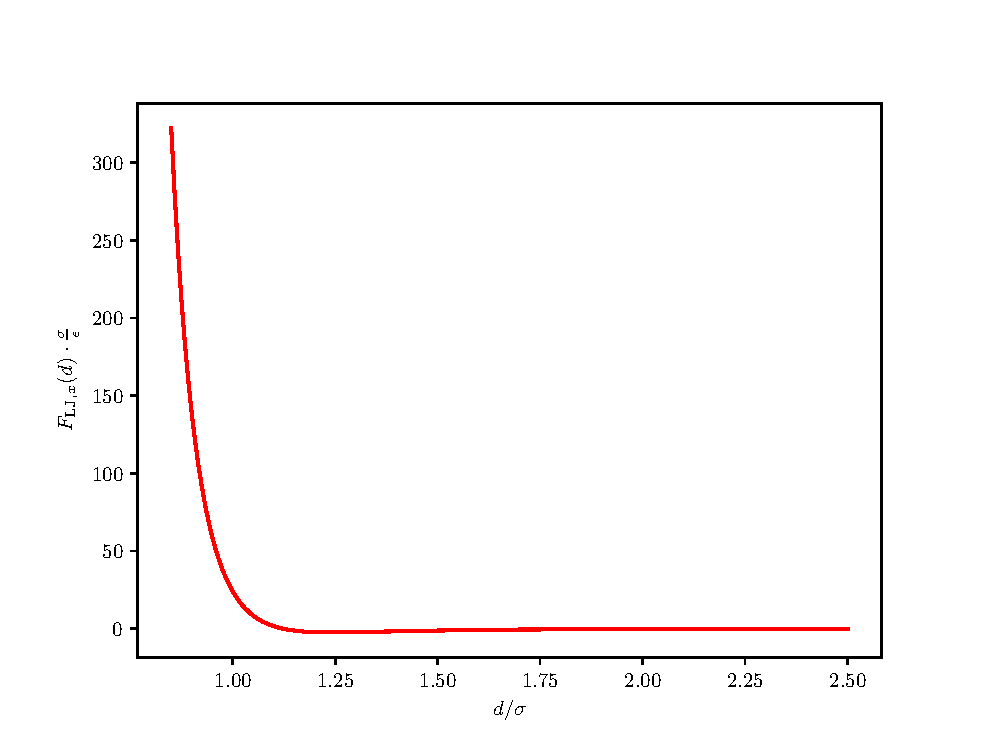
\includegraphics{lennard_jones_force.eps}
 \caption{Plot of the $x$-component of the Lennard-Jones force as a function of the distance $d$.}
 \label{fig:fig2}
\end{figure}

\subsection{Lennard-Jones Billiards}
A plot of the simulated trajectories is shown in .... 
We can see that there already is a collision between the third and fifth particle. 
In contrast to billiard balls, which can be modeled as hard spheres, the Lennard-Jones potential of the particles is not purely repulsive, but also has an attractive part. 
This leads not only to collisions, but also to a situation where two particles circle each other.
For the chosen initial conditions, this can be observed for the second and fourth particle.

\subsection{Periodic Boundary Conditions}
The functions for the truncated Lennard-Jones potential and force where implemented in the following way:
\begin{lstlisting}
def lj_potential(r_ij, R_CUT, SHIFT):
    if np.linalg.norm(r_ij) > R_CUT:
        return 0
    else:
        return ex_3_2.lj_potential(r_ij) - SHIFT
\end{lstlisting}

\begin{lstlisting}
def lj_force(r_ij, R_CUT):
    if np.linalg.norm(r_ij) > R_CUT:
        return 0
    else:
        return ex_3_2.lj_force(r_ij)
\end{lstlisting}
To take into account the periodic boundary conditions with the minimum image convention, we implemented the function pbc:
\begin{lstlisting}
def pbc(x, BOX):
    ret = np.zeros_like(x)
    for dim in range(len(ret)):
        ret[dim] = x[dim] - BOX[dim] * np.rint(x[dim]/ BOX[dim])
    return ret
\end{lstlisting}
This functions has the numpy arrays x and BOX as its input.
x represents a vector like the difference vector $\mathbf{r}_{ij}$ between two particles. 
BOX contains the dimensions of the domain with periodic boundary condition.
The function returns the vector x according to the minimum image convention

\begin{lstlisting}
def minimum_image_vector(x, y, BOX):
    return pbc(y - x, BOX)
\end{lstlisting}




\subsection{Lennard-Jones Fluid}
\subsection{Verlet Lists}

\end{document}
